% !TeX spellcheck = en_GB

% ------------------------------- %
%% Introduction, AdaBoost classifier %%
% ------------------------------- %

%\begin{frame}{The idea behind AdaBoost \,\,i}
%What are we predicting?
%
%$\mathcal{Y}\in\set{-1,1}$
%
%Weak learner, base classifier
%
%\begin{figure}
%%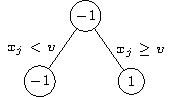
\includegraphics[width=0.3\textwidth,page=1]{./Figures/drawings/drawings.pdf}
%\begin{tikzpicture}[]
%	\tikzset{help lines/.append style=pink}
%	%	\draw [help lines] (-2,-2) grid (2,1);
%	
%	\node[treenode] (root) at (0,0) {$-1$};
%	\node[treenode] (root-l) at (-125:1.35) {$-1$};
%	\node[treenode] (root-r) at (-55:1.35) {$1$};
%	
%	\draw[-] (root) -- node[font=\scriptsize,left] {$x_j<v$} (root-l);
%	\draw[-] (root) -- node[font=\scriptsize,right] {$x_j\geq v$} (root-r);
%\end{tikzpicture}
%\end{figure}
%
%\end{frame}

% ------------------------------- %

%\begin{frame}{The idea behind AdaBoost \,\,i}
%%
%\begin{columns}[T]
%\begin{column}{0.48\textwidth}
%\begin{figure}
%\centering
%\begin{tikzpicture}
%	%draw,ellipse,fill=red!20,minimum height=2em,text centered,font=\sffamily\small
%	\tikzset{help lines/.append style=pink}
%	%\draw [help lines] (-2,-8) grid (3,1);
%
%	\begingroup\linespread{0.95}
%	\node[cloud] (m1) at (0,0) {training data};
%	\node[cloud] (m2) at (0,-1.5) {weighted data};
%	\node[cloud] (M) at (0,-4.5) {weighted data};
%	\endgroup
%	\draw[-latex] (m1) to (m2);
%	\draw[-,dotted,very thick] ($(m2.south) + (0,-0.15)$) to ($(M.north) + (0,+0.15)$);
%	
%	\node (G1) at (2.3,0) {$G_1(x)$};
%	\node (G2) at (2.3,-1.5) {$G_2(x)$};
%	\node (GM) at (2.3,-4.5) {$G_M(x)$};
%	\draw[-stealth] ($(m1.east) + (0.15,0)$) to (G1);
%	\draw[-stealth] ($(m2.east) + (0.15,0)$) to (G2);
%%	\draw[-,dotted] (G2) to (GM);
%	\draw[-stealth] ($(M.east) + (0.15,0)$) to (GM);
%
%%	\node[rectangle,fill=pink!80] (G) at (1.5,-6) {$G(x)=\sign\Bigl(\sum_{m=1}^M\beta_mG_m(x)\Bigr)$};
%	\node[rectangle,fill=mLightGreen!20,font=\large] (G) at (1.6,-6.2) {$G(x)=\sign\Bigl(\lambda\sum_{m=1}^M\alpha_mG_m(x)\Bigr)$};
%%	\draw[-stealth] (GM) to (G);
%\end{tikzpicture}
%\end{figure}
%\end{column}
%\begin{column}{0.48\textwidth}
%\vspace{0.6em}
%Journey to the final classifier:
%{\small\begin{itemize}
%	\setlength{\itemsep}{-0.8ex}
%	\item Linear combination of \alert{weak learners}
%	\item Adaptively build up complexity
%	\item Early stopping to achieve regularization
%	\item \alert{Re-weighting} of training data  % permette all'algoritmo di concentrarsi sugli esempi più difficili da classificare, quindi di questi esempi viene aumentato il peso
%\end{itemize}}
%\vspace{0.8em}
%%Loss function:
%%\[L(y,f(x))=\exp(-yf(x))\]
%Misclassification rate:\vspace{-1ex}
%\[
%\overline{\text{err}}=\frac{1}{N}\sum_{i=1}^N\mathbb{I}(y_i\neq G(x_i))
%\]
%%\begin{figure}
%%\centering
%%\begin{tikzpicture}
%%	\begin{axis}[xlabel=$yf(x)$,ylabel={$L$},axis lines=middle,enlargelimits,width=0.9\textwidth]
%%		\addplot[samples=200,blue,smooth] {exp(-x)};
%%		%\addplot[dashed] {1};
%%%		\addplot [black, mark=-, nodes near coords=$\log(2)$, font={\scriptsize}, every node near coord/.style={anchor=180}] coordinates {(0,{ln(2)})};
%%	\end{axis}
%%\end{tikzpicture}
%%\end{figure}
%\end{column}
%\end{columns}
%
%\end{frame}



\begin{frame}{The idea behind AdaBoost (Discrete AdaBoost)}
%
\begin{columns}[T]
\begin{column}{0.48\textwidth}
\begin{figure}
\centering
\begin{tikzpicture}
	%draw,ellipse,fill=red!20,minimum height=2em,text centered,font=\sffamily\small
	\tikzset{help lines/.append style=pink}
	%\draw [help lines] (-2,-8) grid (3,1);
	
	\begingroup\linespread{0.95}
	\node[cloud] (m1) at (0,0) {training data};
	\node[cloud] (m2) at (0,-1.5) {weighted data};
	\node[cloud] (M) at (0,-4.5) {weighted data};
	\endgroup
	\draw[-latex] (m1) to (m2);
	\draw[-,dotted,very thick] ($(m2.south) + (0,-0.15)$) to ($(M.north) + (0,+0.15)$);
	
	\node (G1) at (2.3,0) {$G_1(x)$};
	\node (G2) at (2.3,-1.5) {$G_2(x)$};
	\node (GM) at (2.3,-4.5) {$G_M(x)$};
	\draw[-stealth] ($(m1.east) + (0.15,0)$) to (G1);
	\draw[-stealth] ($(m2.east) + (0.15,0)$) to (G2);
	%	\draw[-,dotted] (G2) to (GM);
	\draw[-stealth] ($(M.east) + (0.15,0)$) to (GM);
	
	%	\node[rectangle,fill=pink!80] (G) at (1.5,-6) {$G(x)=\sign\Bigl(\sum_{m=1}^M\beta_mG_m(x)\Bigr)$};
	\node[rectangle,fill=mLightGreen!20,font=\large] (G) at (1.6,-6.2) {$G(x)=\sign\Bigl(\sum_{m=1}^M\alpha_mG_m(x)\Bigr)$};
	%	\draw[-stealth] (GM) to (G);
\end{tikzpicture}
\end{figure}
\end{column}
\begin{column}{0.48\textwidth}
\vspace{1em}
Encoding $\mathcal{Y}\in\set{-1,1}$

Base classifier $G_m(x)$ (CART)
\begin{figure}
%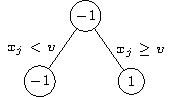
\includegraphics[width=0.3\textwidth,page=1]{./Figures/drawings/drawings.pdf}
\begin{tikzpicture}[]
	\tikzset{help lines/.append style=pink}
	%	\draw [help lines] (-2,-2) grid (2,1);
	
	\node[treenode] (root) at (0,0) {$-1$};
	\node[treenode] (root-l) at (-125:1.35) {$-1$};
	\node[treenode] (root-r) at (-55:1.35) {$1$};
	
	\draw[-] (root) -- node[font=\footnotesize,left] {$x_j<v$} (root-l);
	\draw[-] (root) -- node[font=\footnotesize,right] {$x_j\geq v$} (root-r);
\end{tikzpicture}
\end{figure}

\vspace{1em}
Misclassification rate:\vspace{-1ex}
\[
\overline{\text{err}}=\frac{1}{N}\sum_{i=1}^N\mathbb{I}(y_i\neq G(x_i))
\]

\vspace{-0.7cm}\hspace{-0.25ex}\begin{tikzpicture}
	\tikzset{help lines/.append style=pink}
%	\draw [help lines] (-2,-1) grid (2,1); \node[draw,circle] at (0,0) {};

	\draw[-stealth,bend right=35,thick] (-2,0.3) to (1.7,1.6);
\end{tikzpicture}

\end{column}
\end{columns}

\end{frame}

% ------------------------------- %

\begin{frame}{AdaBoost as an additive model and stochastic setting}
% modello additivo perché in ogni albero c'è soltanto una variabile
\begin{columns}[T]
\begin{column}{0.48\textwidth}
\begin{figure}
\centering
\vspace*{-0.5em}\begin{tikzpicture}
	%draw,ellipse,fill=red!20,minimum height=2em,text centered,font=\sffamily\small
	\tikzset{help lines/.append style=pink}
	%	\draw [help lines] (-2,-8) grid (3,1); \node[draw,circle,red] at (0,0) {};
	
	\node[cloud2] (m1) at (0,0) {$w^{(1)}, \pi_1$};
	\node[cloud2] (m2) at (0,-1.25) {$w^{(2)}, \pi_2$};
	\node[cloud2] (M) at (0,-4.5) {$w^{(M)}, \pi_M$};
	\draw[-latex] (m1) to (m2);
	\draw[-,dotted,very thick] ($(m2.south) + (0,-0.15)$) to ($(M.north) + (0,+0.15)$);
	
	\node (G1) at (2.3,0) {$G_1, f_1$};
	\node (G2) at (2.3,-1.25) {$G_2, f_2$};
	\node (GM) at (2.3,-4.5) {$G_M, f_M$};
	\draw[-stealth] ($(m1.east) + (0.15,0)$) to (G1);
	\draw[-stealth] ($(m2.east) + (0.15,0)$) to (G2);
	%	\draw[-,dotted] (G2) to (GM);
	\draw[-stealth] ($(M.east) + (0.15,0)$) to (GM);
	
	%	\node[rectangle,fill=pink!80] (G) at (1.5,-6) {$G(x)=\sign\Bigl(\sum_{m=1}^M\beta_mG_m(x)\Bigr)$};
%	\node[rectangle,fill=teal!20,font=\large,right] (f) at (-1,-5.55) {$L(y,f(x))=\exp(-yf(x))$};
	\node[rectangle,fill=teal!20,font=\large,right] (G) at (-1,-5.7) {$f_m(x)=f_{m-1}(x)+\lambda\alpha_mG_m(x)$};
	\node[rectangle,fill=mLightGreen!20,font=\large,right] (L) at (-1,-6.5) {$G(x)=\sign(f_M(x))$};
	%	\draw[-stealth] (GM) to (G);
	
	\begingroup\linespread{0.9}
	\node[font=\footnotesize,text width=4em,centered,text centered,inner sep=0pt] (pi) at (2.8,-2.6) {dataset random subsample};
	\endgroup
	\draw[-stealth] (pi) to ($(m2.east) + (-0.25,-0.1)$);
\end{tikzpicture}
\end{figure}
\end{column}
\begin{column}{0.48\textwidth}
\vspace{0.7em}
Journey to the final classifier:
{\footnotesize\begin{itemize}
	\setlength{\itemsep}{-0.8ex}
	\item Linear combination of \alert{weak learners} (additive model)
	\item Adaptively build up complexity, through a prediction function
	\item Regularization with early stopping and shrinkage
	\item \alert{Re-weighting} of a bootstrapped fraction of the training data  % permette all'algoritmo di concentrarsi sugli esempi più difficili da classificare, quindi di questi esempi viene aumentato il peso
\end{itemize}}
%$f_m(x)$ prediction function

%$\lambda$ shrinkage coefficient


\vspace{0.8em}
Exponential loss function:\vspace{-1ex}
\[L(y,f(x))=\exp(-yf(x))\]
%\begin{figure}
%\centering
%\begin{tikzpicture}
%	\begin{axis}[xlabel=$yf(x)$,ylabel={$L$},axis lines=middle,enlargelimits,width=1.2\textwidth]
%		\addplot[samples=200,blue,smooth] {exp(-x)};
%		%\addplot[dashed] {1};
%%		\addplot [black, mark=-, nodes near coords=$\log(2)$, font={\scriptsize}, every node near coord/.style={anchor=180}] coordinates {(0,{ln(2)})};
%	\end{axis}
%\end{tikzpicture}
%\end{figure}
\end{column}
\end{columns}

\end{frame}

% ------------------------------- %

\begin{frame}{AdaBoost in practice}
\vspace*{-2.5em}\lstinline|ada::ada(formula, data, loss="exponential", type="discrete", iter, nu=0.01, bag.frac)|\bigskip\smallskip

\begin{columns}[T]
\begin{column}{0.5\textwidth}
Function \texttt{ada} arguments:\vspace{-1ex}
{\small\begin{itemize}
	\setlength{\itemsep}{-0.8ex}
	\item \texttt{loss}: boosting loss function
	\item \texttt{type}: AdaBoost version
	\item \texttt{iter}: boosting rounds
	\item \texttt{nu}: shrinkage coefficient $\lambda$
	\item \texttt{bag.frac}: in-bag fraction \numlist{1;0.5}
\end{itemize}}
\end{column}
\begin{column}{0.5\textwidth}
%Journey to the final classifier:
%{\small\begin{itemize}
%\setlength{\itemsep}{-0.8ex}
%\item Linear combination of \alert{weak learners} (additive model)
%\item Adaptively build up complexity, through a prediction function
%\item Regularization with early stopping and shrinkage
%\item \alert{Re-weighting} of a subsample of the training data  % permette all'algoritmo di concentrarsi sugli esempi più difficili da classificare, quindi di questi esempi viene aumentato il peso
%\end{itemize}}
\begin{figure}
% quando è classificato correttamente y e f(x) avranno segno concorde, la funzione andrà a 0
% quando il label non è corretto, il segno discorde manda la funzione a infinito
\begin{tikzpicture}
\begin{axis}[xlabel=$yf(x)$,ylabel={$L(y,f(x))$},axis lines=middle,enlargelimits,width=1.1\textwidth,tick label style={font=\scriptsize}]
	\addplot[samples=200,blue,smooth,thick] {exp(-x)};
	%\addplot[dashed] {1};
\end{axis}
\end{tikzpicture}
\end{figure}
\end{column}
\end{columns}

\end{frame}




%\begin{frame}{coide}
%
%{\footnotesize Package \texttt{\{randomForest\}}\vspace{-1ex}
%\begin{itemize}\setlength{\itemsep}{-0.5ex}
%	\item \texttt{randomForest(formula, data={\color{blue}NULL}, ntree={\color{red}500}, mtry={\color{blue}sqrt}(p), importance={\color{red}TRUE}, \dots)}
%	\item \lstinline|randomForest(formula, data=NULL, ntree=500, mtry=sqrt(p), importance=TRUE)|
%	\item \texttt{importance(x, type={\color{blue}NULL}, class={\color{blue}NULL}, \dots)}
%	\item \texttt{varImpPlot(x, sort={\color{red}TRUE}, \dots)}
%	\item \texttt{rf.model\$confusion}
%	\item \texttt{rf.model\$err.rate}
%\end{itemize}}
%\end{frame}

